% TinyAudit -- workshop paper scaffold.
% Target: NeurIPS Responsible AI workshop 2026 (reach: ACM FAccT 2027).
% This is a portable `article` skeleton so it builds anywhere; to submit, swap
% \documentclass for the venue style file and move the abstract/authors into it.
%
% Every number in the tables below is a mean +/- std over 10 seeds, taken from
% experiments/results/*_multiseed.csv. Do not hand-edit numbers here; regenerate
% the CSVs (python experiments/run_multiseed.py) and update the tables.
%
% \todo{...} marks where prose still needs to be written.

\documentclass[11pt]{article}

\usepackage[margin=1in]{geometry}
\usepackage{booktabs}
\usepackage{graphicx}
\usepackage{amsmath}
\usepackage{xcolor}
\usepackage{hyperref}
\usepackage{siunitx}

\newcommand{\todo}[1]{{\color{red}\textbf{[TODO: #1]}}}
\newcommand{\dataset}[1]{\textsc{#1}}

\title{TinyAudit: On-Device, Uncertainty-Aware Fairness Audits\\
Survive (and Expose) Compression}
\author{Atharva Doke \and Kasyap Tumuluri}
\date{\today}

\begin{document}
\maketitle

\begin{abstract}
Machine learning is moving onto microcontroller-class hardware, where models are
aggressively compressed (pruned, quantized) to fit. Responsible-AI audits, in
contrast, are almost always run on full-precision models on a workstation, and
they typically look at fairness, uncertainty, and explainability in isolation. We
present \textsc{TinyAudit}, an auditing pipeline that measures all three together
\emph{through} compression and \emph{within} the memory and compute envelope of
the audited model itself. Using it we report two findings, each replicated and
reported as a mean over 10 seeds. First, point-prediction fairness and
calibration fairness are \emph{decoupled}: the two lenses rank sensitive groups
differently, so a model that looks fair on demographic parity need not be fair in
its per-group calibration. The result holds on \dataset{UCI Adult} and replicates
on \dataset{COMPAS}, whose favorable direction is inverted. Second, compression
can \emph{hide} unfairness: as a network is pruned it can look progressively
fairer on demographic parity precisely as its calibration collapses, because it
degrades toward a near-constant predictor. \todo{one sentence on the on-device
feasibility result once the audit-footprint number is finalized.}
\end{abstract}

\section{Introduction}
\label{sec:intro}

Two trends collide. \todo{expand: (1) ML on microcontroller-class hardware, where
models are compressed to fit; (2) responsible-AI audits run offline, full
precision, one axis at a time. Nobody checks what compression does to audit
properties, or whether the audit fits the device budget.}

\paragraph{The claim.} Compression-era model audits must be uncertainty-aware:
point-fairness and calibration-fairness are decoupled, and compression can move
one without the other, and this can be measured within the device's own compute
budget.

\paragraph{Contributions.}
\begin{enumerate}
    \item An auditing pipeline that couples fairness, uncertainty, and
    explainability and measures them on the \emph{compressed} model, inside an
    on-device budget (Section~\ref{sec:instrument}).
    \item A decoupling result: point-fairness and calibration-fairness rank
    sensitive groups differently, on \dataset{Adult} and replicated on
    \dataset{COMPAS} (Section~\ref{sec:decoupling}).
    \item Evidence that compression can hide unfairness: demographic parity and
    calibration move in opposite directions under pruning
    (Section~\ref{sec:compression}).
    \item \todo{the feasibility claim: the audit runs in X of budget
    (Section~\ref{sec:feasibility}).}
\end{enumerate}

\section{The TinyAudit Instrument}
\label{sec:instrument}

Given a fitted model and a labeled test set, \textsc{TinyAudit} runs a seven-stage
pipeline and emits a one-page audit card plus a machine-readable manifest:
(1) profile (parameters, FLOPs, peak RAM, wall-clock); (2) point fairness
(demographic parity, equalized odds, disparate impact); (3) uncertainty (MC
dropout, a perturbation ensemble, early exit); (4) uncertainty-aware fairness
(per-group predictive entropy, per-group expected calibration error, selective
fairness); (5) explainability (SHAP, LIME, occlusion); (6) compression (int8
quantization or magnitude pruning, applied \emph{before} the metrics above);
(7) render. \todo{expand each stage briefly; state the budget constraint and how
it is enforced. Cite docs/architecture.md.}

\section{Experimental Setup}
\label{sec:setup}

\paragraph{Datasets and models.} We use \dataset{UCI Adult}, \dataset{COMPAS},
and the \dataset{ACSIncome} subset of \dataset{Folktables} (real 2018 California
Census data). Models are standard scikit-learn estimators: logistic regression,
a two-hidden-layer MLP, and a decision tree, each fit on \texttt{StandardScaler}d
features. \todo{justify scaling: without it the MLP on Adult is unusable
($\approx 0.54$ accuracy); with it, $\approx 0.84$.} Sensitive attributes are
\texttt{sex} and \texttt{race}.

\paragraph{Reproducibility.} A single \texttt{seed} flag seeds every RNG. All
headline numbers are reported as mean $\pm$ standard deviation over seeds 0--9
(\texttt{experiments/run\_multiseed.py}); every result CSV is stamped with the
seed, a config hash, and resolved library versions. Determinism is guaranteed on
Linux/x86; minor float drift elsewhere is expected, which is why the std columns
matter.

\paragraph{Baselines.} Table~\ref{tab:baselines} confirms the models are credible
(published-range accuracy), so the fairness findings sit on top of models that
work.

\begin{table}[t]
\centering
\caption{Baseline model quality (mean $\pm$ std over 10 seeds).
Source: \texttt{baselines\_multiseed.csv}.}
\label{tab:baselines}
\begin{tabular}{llccr}
\toprule
Dataset & Model & Accuracy & ROC-AUC & Params \\
\midrule
Adult      & logreg & $0.852 \pm 0.003$ & $0.906 \pm 0.002$ & 102 \\
Adult      & MLP    & $0.837 \pm 0.003$ & $0.884 \pm 0.003$ & 4{,}353 \\
Adult      & tree   & $0.817 \pm 0.003$ & $0.751 \pm 0.005$ & 10{,}720 \\
COMPAS     & logreg & $0.680 \pm 0.006$ & $0.731 \pm 0.008$ & 6 \\
COMPAS     & MLP    & $0.683 \pm 0.008$ & $0.736 \pm 0.009$ & 1{,}281 \\
ACSIncome  & logreg & $0.781 \pm 0.001$ & $0.856 \pm 0.001$ & 9 \\
ACSIncome  & MLP    & $0.808 \pm 0.003$ & $0.889 \pm 0.002$ & 1{,}377 \\
\bottomrule
\end{tabular}
\end{table}

\section{Finding 1: The Fairness Lenses Decouple}
\label{sec:decoupling}

\todo{state the finding in one sentence, then walk the tables.} On \dataset{Adult}
by \texttt{race} (Table~\ref{tab:decoup-adult}), the best-calibrated group by a
wide margin (White, ECE $0.008 \pm 0.002$) is one of the most-selected, not the
worst served by the point predictions, so the selection-rate ranking and the
calibration ranking do not line up; the smaller groups carry higher, noisier
calibration error the selection view never surfaces. By \texttt{sex}, the
Male/Female gap is large in selection rate ($0.253 \pm 0.007$ vs
$0.079 \pm 0.004$) but negligible in calibration ($0.009$ vs $0.014$).

The result replicates on \dataset{COMPAS} (Table~\ref{tab:decoup-compas}), where
the positive outcome is being flagged high-risk (higher is worse). African-American
defendants are flagged at roughly twice the rate of the next group
($0.441$ vs $0.249$), yet the worst-calibrated group is the one flagged
\emph{least}. Point parity and calibration parity single out different groups on a
second dataset whose favorable direction is inverted, so the finding is not an
\dataset{Adult}-specific artifact.

\begin{table}[t]
\centering
\caption{\dataset{Adult} $\times$ \texttt{race}, uncompressed logistic model
(mean $\pm$ std, 10 seeds). Source: \texttt{decoupling\_adult\_multiseed.csv}.}
\label{tab:decoup-adult}
\begin{tabular}{lccc}
\toprule
Group (race) & Selection rate & Mean entropy & ECE \\
\midrule
Asian-Pac-Islander & $0.240 \pm 0.014$ & $0.318 \pm 0.010$ & $0.037 \pm 0.014$ \\
White              & $0.207 \pm 0.005$ & $0.337 \pm 0.007$ & $\mathbf{0.008 \pm 0.002}$ \\
Amer-Indian-Eskimo & $0.098 \pm 0.026$ & $0.287 \pm 0.025$ & $0.056 \pm 0.019$ \\
Black              & $0.091 \pm 0.008$ & $0.235 \pm 0.009$ & $0.024 \pm 0.006$ \\
Other              & $0.081 \pm 0.024$ & $0.223 \pm 0.020$ & $0.046 \pm 0.016$ \\
\bottomrule
\end{tabular}
\end{table}

\begin{table}[t]
\centering
\caption{\dataset{COMPAS} $\times$ \texttt{race}, uncompressed logistic model
(mean $\pm$ std, 10 seeds; two groups with $n<10$ omitted). Positive outcome =
flagged high-risk. Source: \texttt{decoupling\_compas\_multiseed.csv}.}
\label{tab:decoup-compas}
\begin{tabular}{lcc}
\toprule
Group (race) & High-risk flag rate & ECE \\
\midrule
African-American & $\mathbf{0.441 \pm 0.015}$ & $0.057 \pm 0.010$ \\
Hispanic         & $0.249 \pm 0.046$ & $0.068 \pm 0.024$ \\
Caucasian        & $0.227 \pm 0.013$ & $\mathbf{0.035 \pm 0.016}$ \\
Other            & $0.164 \pm 0.033$ & $\mathbf{0.094 \pm 0.029}$ \\
\bottomrule
\end{tabular}
\end{table}

\section{Finding 2: Compression Can Hide Unfairness}
\label{sec:compression}

As the \dataset{Adult} MLP is pruned from uncompressed to 90\% sparsity
(Table~\ref{tab:compression}), its demographic-parity gap net falls
($0.175 \rightarrow 0.014$) while per-group calibration error net climbs roughly
tenfold ($0.027 \rightarrow 0.282$): the model looks fairer on parity precisely as
its calibration collapses, because it degrades toward a near-constant predictor.
\todo{emphasize this is an endpoint contrast: the intermediate pruning levels are
seed-noisy (parity std $\pm 0.06$ to $\pm 0.10$), so the direction is the robust
claim. Add Figure~\ref{fig:compression} with the error bands.}

\begin{table}[t]
\centering
\caption{\dataset{Adult} MLP, \texttt{sex}, over pruning sparsity
(mean $\pm$ std, 10 seeds). Source: \texttt{compression\_sweep\_multiseed.csv}.}
\label{tab:compression}
\begin{tabular}{lcc}
\toprule
Pruning & Demographic-parity diff & Per-group ECE \\
\midrule
none      & $0.175 \pm 0.016$ & $0.027 \pm 0.006$ \\
30\%      & $0.181 \pm 0.096$ & $0.194 \pm 0.108$ \\
50\%      & $0.136 \pm 0.080$ & $0.193 \pm 0.100$ \\
70\%      & $0.084 \pm 0.064$ & $0.250 \pm 0.133$ \\
90\%      & $0.014 \pm 0.028$ & $0.282 \pm 0.106$ \\
\bottomrule
\end{tabular}
\end{table}

\begin{figure}[t]
\centering
% 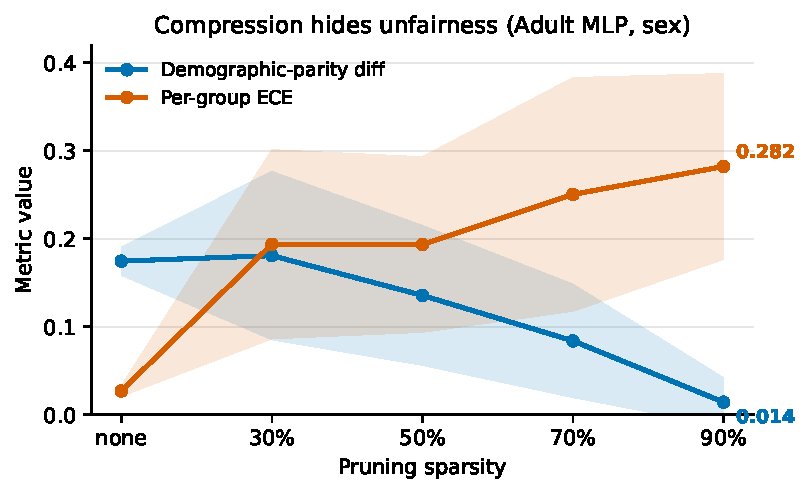
\includegraphics[width=0.7\linewidth]{figures/compression.pdf}
\fbox{\parbox{0.7\linewidth}{\centering \vspace{2cm} \todo{export the crossing
demographic-parity / ECE lines with $\pm 1$ std bands as figures/compression.pdf
(the web one-pager renders the same chart).} \vspace{2cm}}}
\caption{Compression hides unfairness: parity falls as ECE rises; the bands are
$\pm 1$ std over 10 seeds and overlap in the middle, so read the endpoints.}
\label{fig:compression}
\end{figure}

\section{On-Device Feasibility}
\label{sec:feasibility}

\todo{This is the differentiating claim and needs the audit's own footprint, not
just the model's. Table~\ref{tab:footprint} reports the audited models' footprint
(from the profile stage); measure and add the peak RAM / FLOPs of the audit
\emph{pipeline} so the ``fits the device budget'' claim is quantitative.}

\begin{table}[t]
\centering
\caption{Audited-model footprint (mean over 10 seeds).
Source: \texttt{baselines\_multiseed.csv}.}
\label{tab:footprint}
\begin{tabular}{llrrr}
\toprule
Dataset & Model & Params & FLOPs & Peak RAM (KB) \\
\midrule
Adult      & logreg & 102   & 1.2M  & 335 \\
Adult      & MLP    & 4{,}353 & 53M & 6{,}107 \\
COMPAS     & logreg & 6     & 9.3k  & 62 \\
ACSIncome  & MLP    & 1{,}377 & 67M & 24{,}460 \\
\bottomrule
\end{tabular}
\end{table}

\section{Related Work}
\label{sec:related}
\todo{three short paragraphs: (1) uncertainty-aware fairness (the origin of the
decoupling claim); (2) fairness under compression / pruning / quantization;
(3) on-device / TinyML auditing. Say what is new: we couple all three and measure
through compression within the device budget.}

\section{Limitations}
\label{sec:limitations}
\begin{itemize}
    \item Features are standardized before fitting; without it the MLP is unusable.
    \item The uncertainty ``ensemble'' is five lightly-jittered copies of the one
    (compressed) model, not five from-scratch retrains, so read uncertainty
    magnitudes as relative.
    \item int8 models' float weights are unreachable, so their uncertainty columns
    are blank; decision trees have no dense weights and sit out the compression
    grid.
    \item Heavily-pruned \dataset{COMPAS} (only $\approx 5$ features) degenerates
    to a near-constant predictor; read those cells as a corner case.
    \item Exact reproducibility is guaranteed on Linux/x86; elsewhere expect
    last-digit float drift.
\end{itemize}

\section{Conclusion}
\label{sec:conclusion}
\todo{restate the claim and the two findings; point to the released instrument.}

\bibliographystyle{plain}
\bibliography{refs}

\end{document}
